\section{Background and Methodology}

\label{sec:background_cwv} 
\subsection{Core Web Vitals}
Core Web Vitals (CWVs) are standardized, user-centric performance metrics introduced by Google to quantify real-world web experience along three dimensions: \textbf{Largest Contentful Paint (LCP)}, which captures perceived load speed; \textbf{Cumulative Layout Shift (CLS)}, which measures visual stability during page load; and \textbf{Interaction to Next Paint (INP)}, which reflects responsiveness to user interaction.\footnote{\url{https://web.dev/vitals/}}. In this work, the \emph{unit of evaluation is a webpage}: a single URL whose CWVs are measured end-to-end in a browser. A \emph{website} (repository) contributes multiple webpages (the homepage plus a bounded set of internal pages), enabling evaluation across heterogeneous page templates while keeping runtime tractable. Google rates LCP under 2.5\,s, CLS below 0.1, and INP under 200\,ms as ``good''; together, these thresholds span loading, visual stability, and responsiveness. Since 2021 CWVs feed directly into Google's page-experience ranking signal, and poor scores correlate with higher bounce rates and lower conversion~\footnote{\url{https://www.relevantaudience.com/seo/core-web-vitals-and-their-impact-on-seo-ranking/}}, giving site operators strong incentives to optimize. The Chrome User Experience Report (\textbf{CrUX}) aggregates anonymized real-user measurements across millions of origins, reporting p75 distributions over a rolling 28-day window, and serves as the authoritative field-data reference for CWV compliance.\footnote{\url{https://developer.chrome.com/docs/crux}}

Optimizing CWVs is nonetheless difficult: the three metrics interact (e.g.\ deferring JavaScript may improve INP but delay LCP), bottlenecks depend on the critical rendering path which varies across page templates, devices, and networks, and effective fixes often require cross-cutting changes (resource hints, code splitting, lazy loading, font subsetting) that demand understanding of the full frontend stack.


CWVs are attractive as an evaluation target because they capture how users experience deployed webpages, but they also introduce methodological challenges. First, CWV measurements exhibit variance due to nondeterminism in browser scheduling, asynchronous resource loading, and network effects. Second, optimizing CWVs creates incentives for reward hacking (e.g., removing visible content, disabling scripts, or breaking interactive functionality to lower measured latency). Third, because CWVs are often reported as ``field'' metrics derived from real users, a benchmark based on ``lab'' (synthetic) measurement must be designed to align closely with field behavior to remain faithful to real-world impact.

These considerations imply that an execution-based CWV benchmark should provide: (i) a large and diverse set of websites and webpages, (ii) a controlled, safe, and reproducible hosting and measurement environment, (iii) repeated measurement with robust aggregation, and (iv) explicit regression and anti-hacking checks that preserve page semantics and visible content. We next describe \OurBench and the curation and evaluation harness that satisfy these requirements.

\subsection{\OurBench}

\begin{figure}[t]
  \centering
  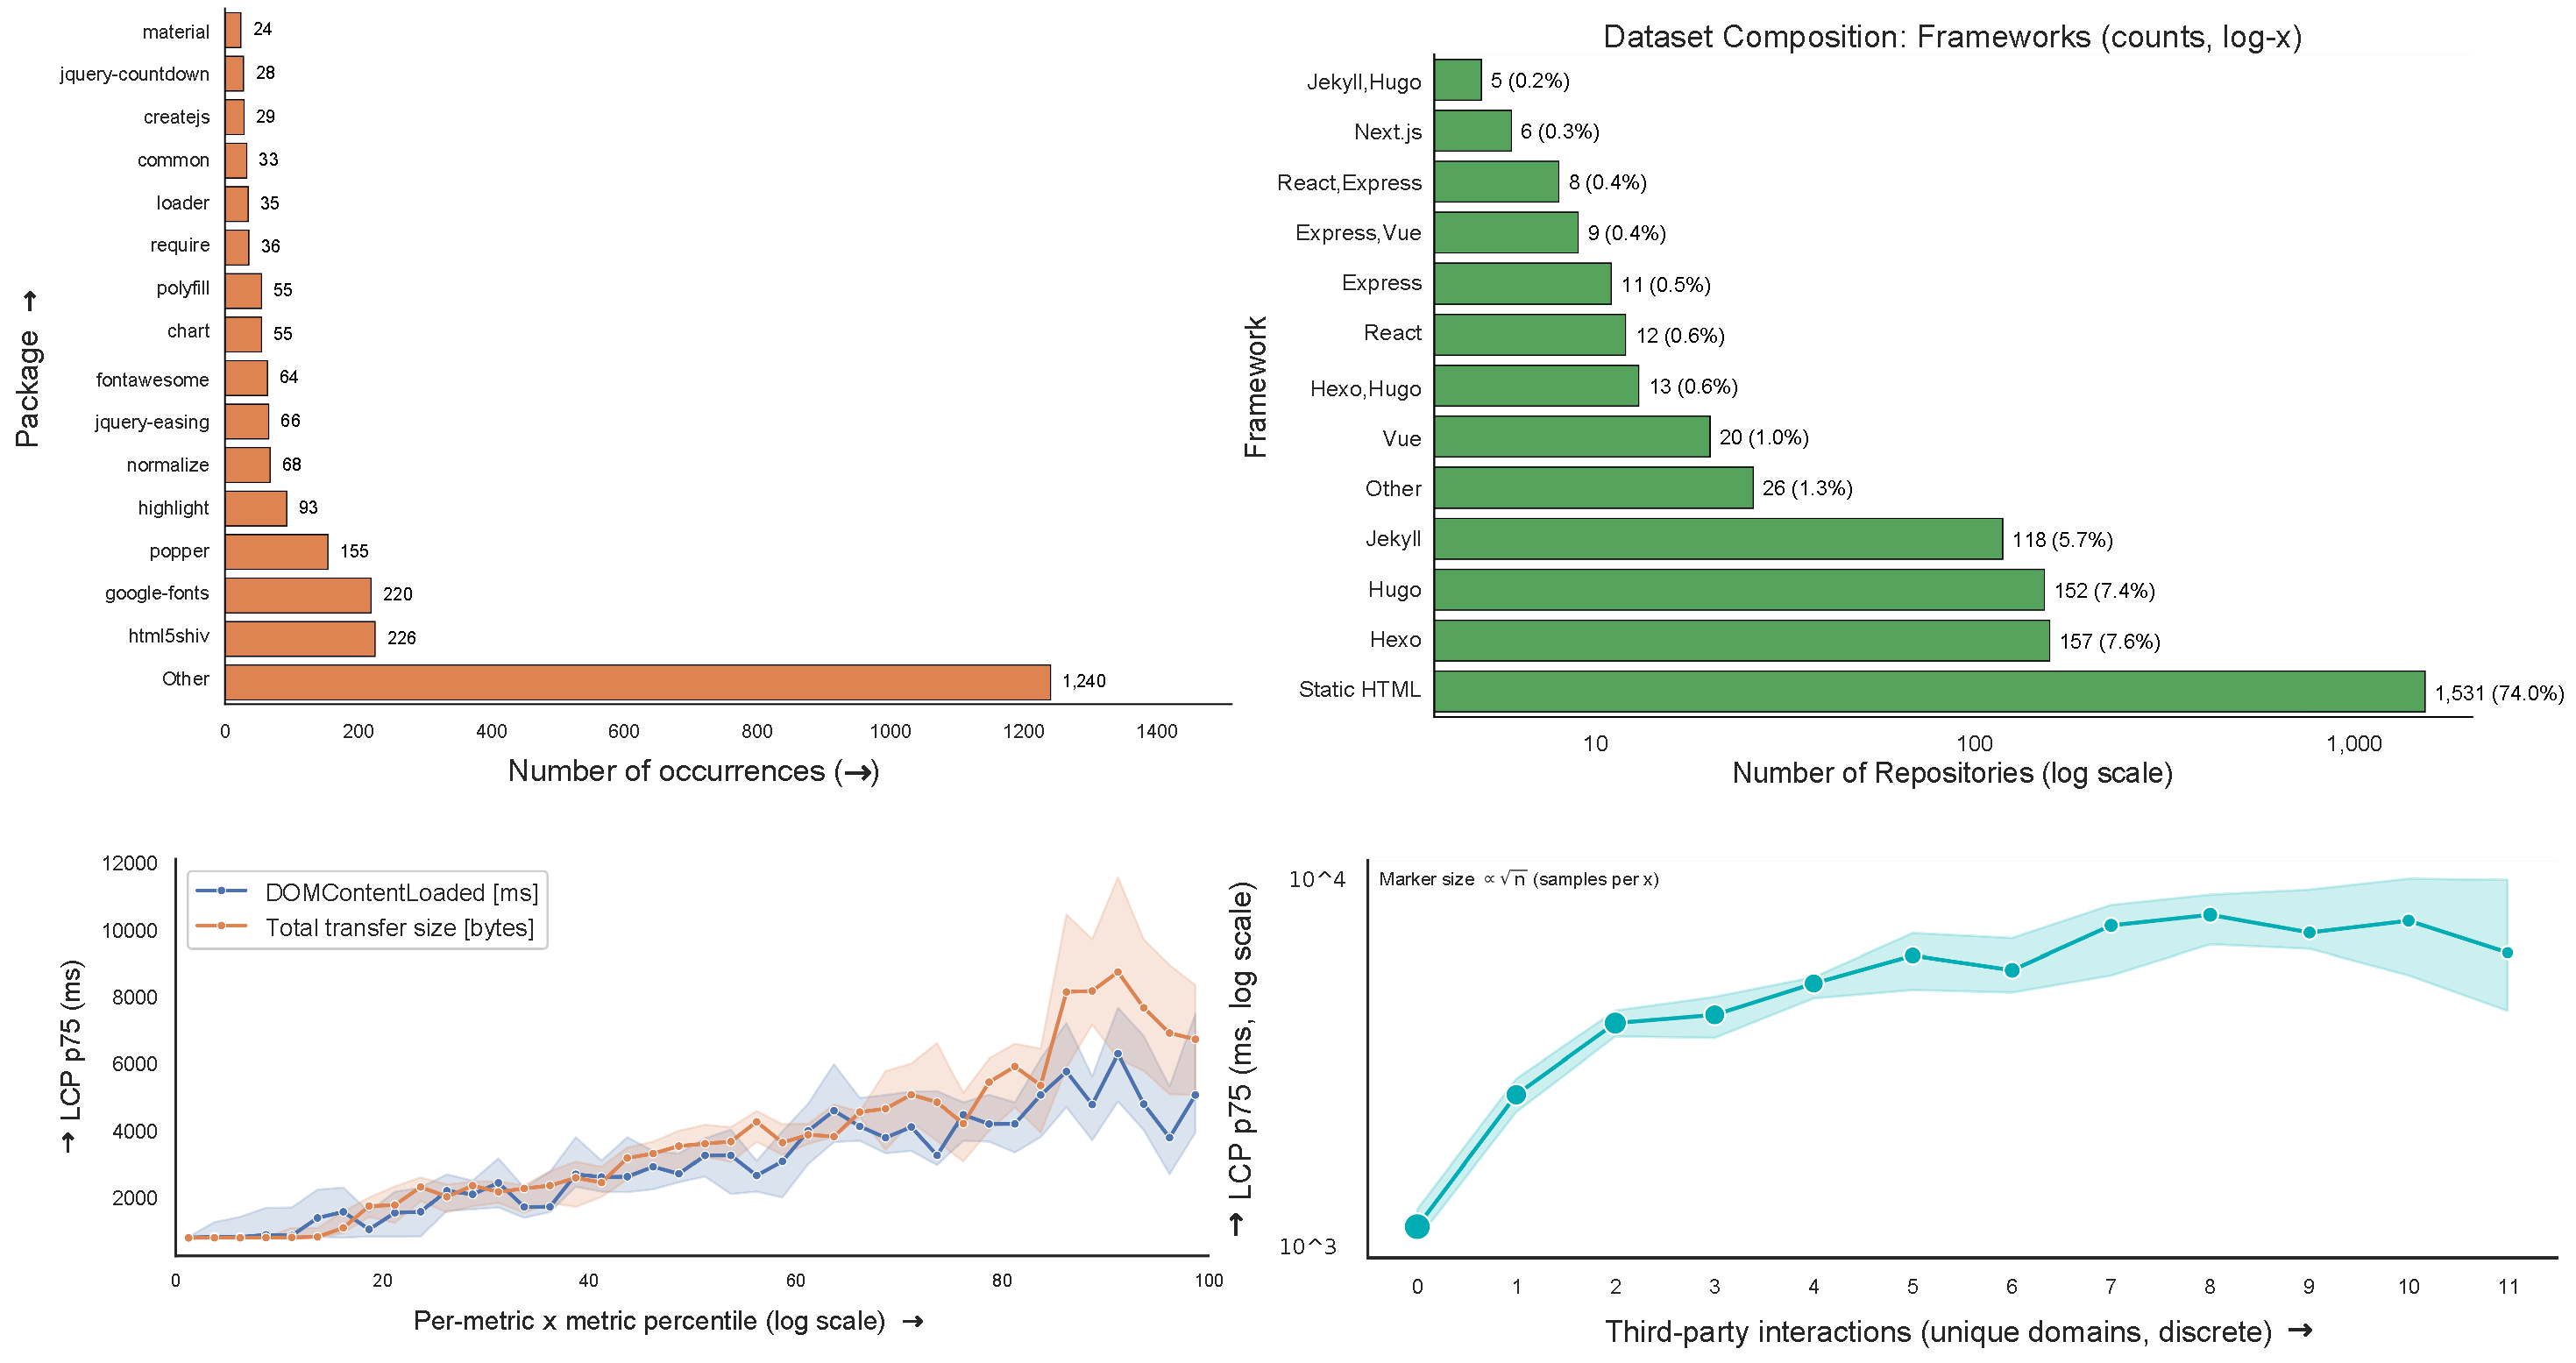
\includegraphics[width=\linewidth]{figures/EDA_PLOTS.pdf}
  \caption{\textbf{Exploratory dataset statistics.}
  \textbf{Top-left:} third-party package frequency (long-tailed).
  \textbf{Top-right:} framework distribution (log scale); Static HTML dominates, followed by Hexo/Hugo/Jekyll.
  \textbf{Bottom-left:} transfer size and \texttt{DOMContentLoaded} rise together toward higher percentiles.
  \textbf{Bottom-right:} LCP p75 increases with third-party domain count, then plateaus.}
  \Description{A four-panel exploratory data figure. The top-left panel shows a long-tailed package frequency distribution. The top-right panel shows framework counts on a log scale with Static HTML as the largest category. The bottom-left panel shows transfer size increasing with DOMContentLoaded. The bottom-right panel shows LCP p75 increasing with third-party domain count before flattening.}
  \label{fig:eda_plots}
\end{figure}


\OurBench is an execution-based benchmark for evaluating coding agents on \emph{goal-directed website performance optimization}. Each benchmark instance consists of: (i) the pinned snapshot or source code for a website, (ii) a deterministic local deployment script that serves the site on localhost, and (iii) a set of webpages on the same origin used for evaluation. Agents may freely modify the repository, and succeed by improving CWVs under strict non-regression constraints, rather than matching a reference patch. Figure~\ref{fig:curation_pipeline} summarizes the end-to-end benchmark curation pipeline.
\begin{figure}[t]
  \centering
  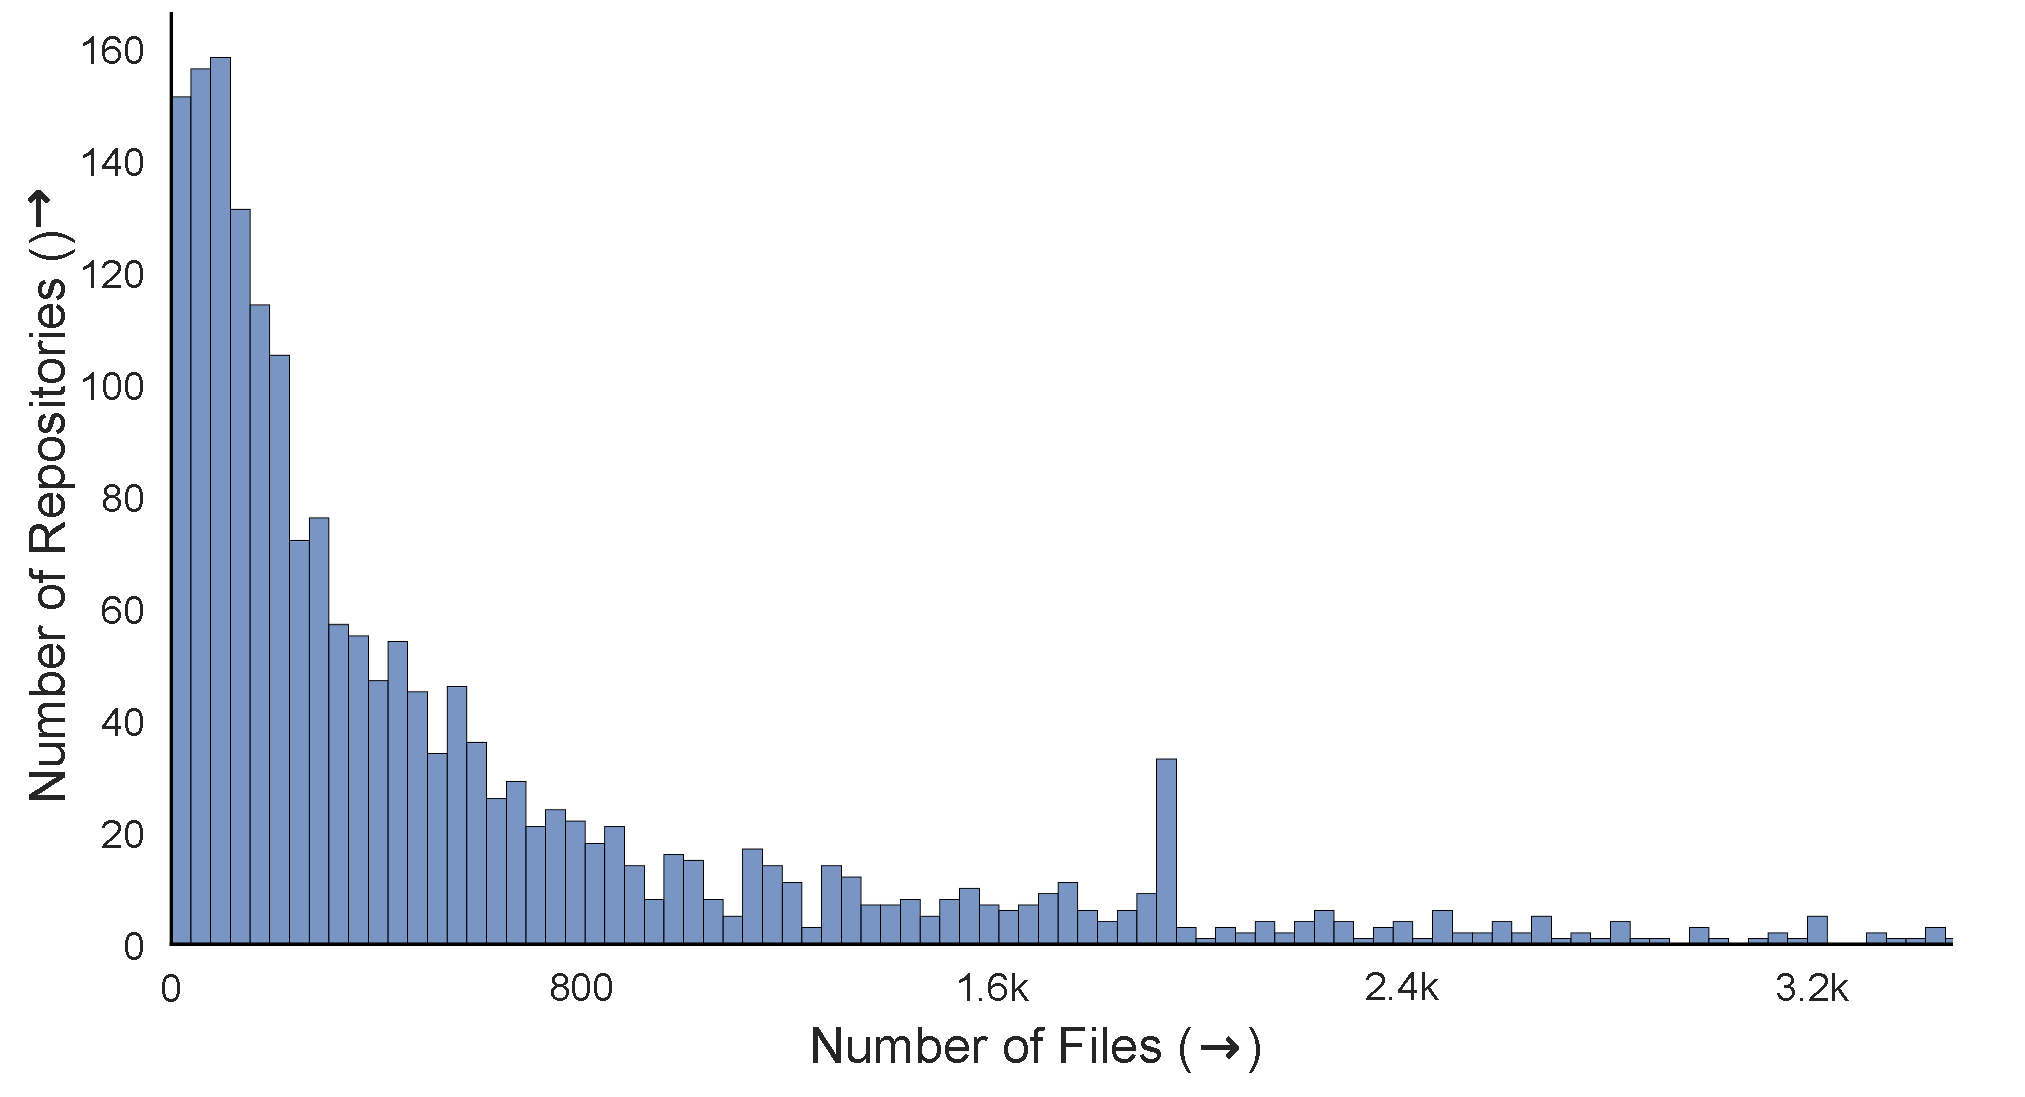
\includegraphics[width=\columnwidth]{figures/FILES_EDA.pdf}
  \caption{\textbf{Repository size distribution (final benchmark).}
  Histogram of the number of files per repository. The distribution is strongly right-skewed: most repositories contain relatively few files, while a small fraction are much larger (long tail reaching into the thousands of files), indicating substantial variability in repo scale.}
  \Description{A histogram of repository file counts in the final benchmark. Most repositories have relatively few files, while a long right tail extends to much larger projects with hundreds or thousands of files.}
  \label{fig:files_eda}
\end{figure}



\begin{figure*}[t]
  \centering  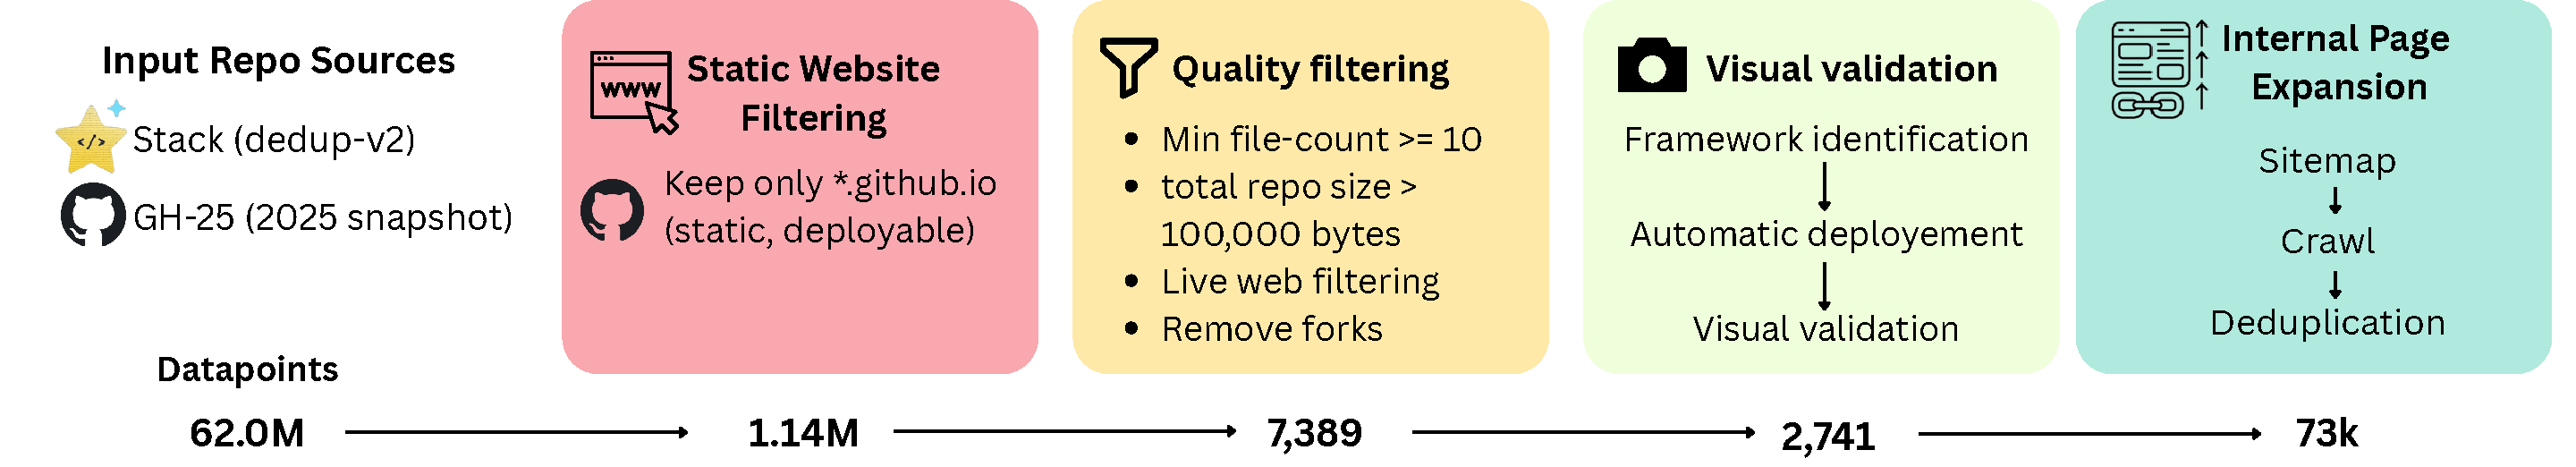
\includegraphics[width=\textwidth]{figures/Benchmark_construction.pdf}
    \caption{Benchmark curation pipeline: Starting from large-scale GitHub repository corpora (Stack dedup-v2 and GH-25), we retain deployable GitHub Pages sites (\texttt{*.github.io}), apply deterministic quality filters, identify frameworks and assign deterministic deployment scripts, validate local deployments against the corresponding live GitHub Pages rendering, and expand each task with bounded internal page discovery and template-level deduplication. The final benchmark contains 2{,}741 repositories and 73k deduplicated internal webpages.}
  \Description{A benchmark curation pipeline diagram. Large repository corpora are filtered to GitHub Pages sites, passed through quality filtering, framework identification, deterministic deployment assignment, live-versus-local validation, and internal page discovery with deduplication, yielding the final benchmark of validated repositories and internal webpages.}
  \label{fig:curation_pipeline}
\end{figure*}
\begin{figure}[t]
    \centering
    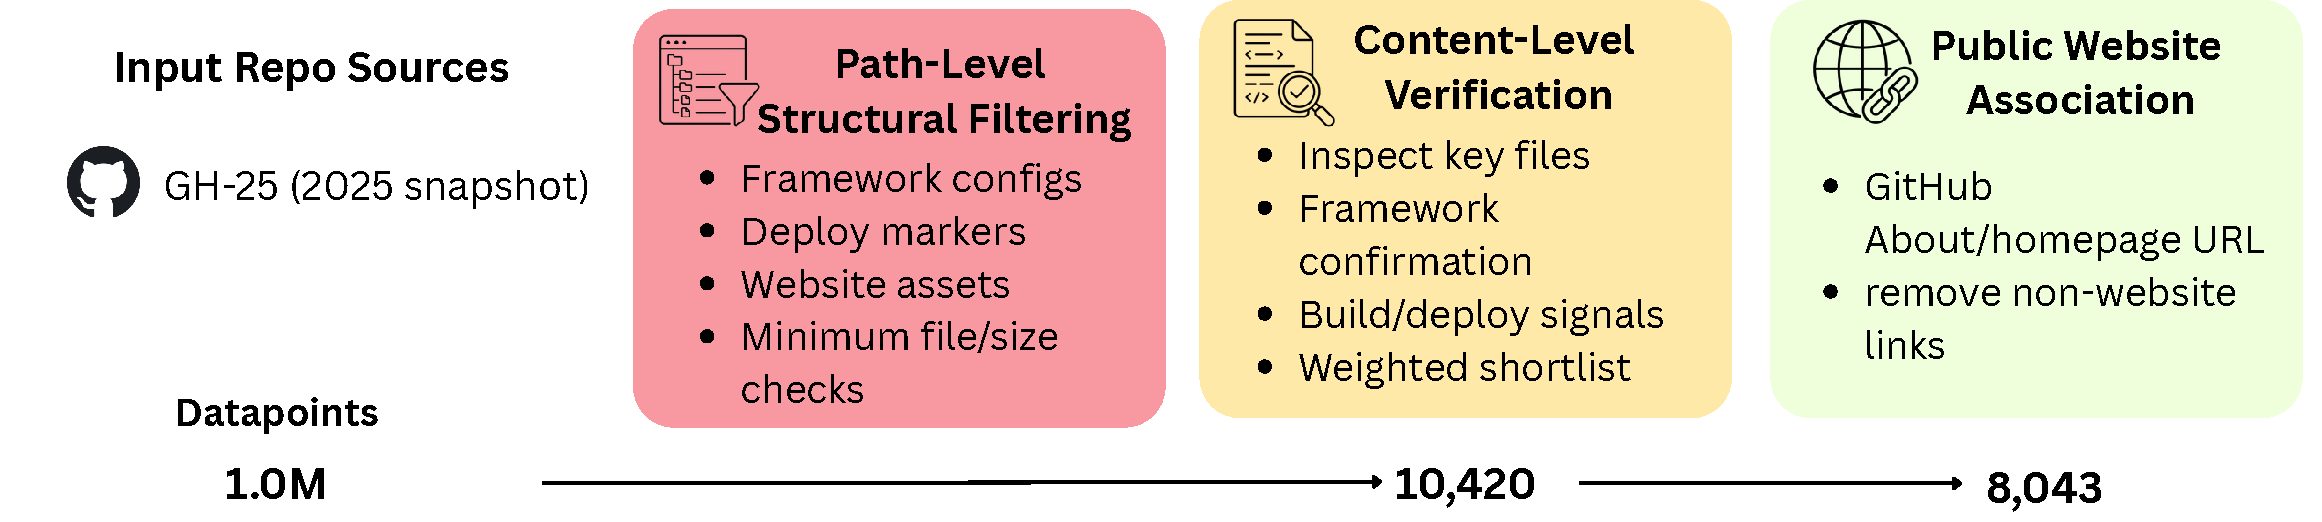
\includegraphics[width=\linewidth]{figures/GH25_Repo_Filtering.pdf} 
    \caption{
    GH-25 three-stage repository filtering pipeline. Starting from approximately 1.0M repositories in the GH-25 snapshot, we first apply path-level structural filtering to identify repositories that resemble web projects. We then perform content-level verification over informative files to confirm framework, build, and deployment signals, producing 10,420 candidate repositories. Finally, we retain repositories associated with a valid public website through the GitHub About/homepage field and deduplicate by homepage URL, yielding 8,043 website candidates for downstream deployment and CWV benchmarking.
    }
    \label{fig:gh25_filtering_pipeline}
\end{figure}
\subsubsection{Repository Sources}
\label{sec:bench_sources}

We source candidate repositories from two public corpora with complementary roles: \textbf{GH-25}\cite{nick007x_github_code_2025}, a 2025 snapshot of 1.5M GitHub repositories, and \textbf{Stack (dedup-v2)}\cite{Kocetkov2022TheStack}, a large-scale deduplicated snapshot of 60M+ GitHub repositories maintained through 2024. GH-25 is the primary source for our main benchmark because SWE-Experience-Bench is intended to evaluate coding agents on contemporary website optimization tasks. Web development changes rapidly: frontend frameworks, build systems, package managers, static-site generators, hosting conventions, and performance anti-patterns evolve continuously. A recent 2025 snapshot therefore gives us a candidate pool that better reflects the current web ecosystem and supports our goal of making the benchmark refreshable over time.

Our curation objective is to find repositories that are likely to represent real, source-backed websites. This distinction matters because each benchmark instance must eventually be locally deployed, rendered in a browser, and measured for Core Web Vitals (CWVs). We therefore prioritize repositories corresponding to frontend applications, static websites, documentation sites, blogs, portfolios, and similar web artifacts, where the source code directly controls the user-facing experience being optimized. These repositories expose the frontend critical path that determines CWV behavior, including resource loading, script execution, layout stability, image and font loading, and interaction responsiveness.

Alongside GH-25, we use Stack (dedup-v2) as an archival complement. Stack provides broad historical coverage of public GitHub repositories and is useful for recovering older GitHub Pages websites that may not be well represented in a newer snapshot. For this archival branch, we focus on repositories associated with \texttt{*.github.io} pages, since the GitHub Pages namespace provides a simple and interpretable link between a repository and a public static website. After applying tractability and quality filters, the Stack branch contributes a validated archival pool, while GH-25 remains the primary source for the main, refreshable benchmark. Together, the two sources let us combine recency with historical breadth: GH-25 captures the current web development landscape, and Stack provides a large archival reference set of public static websites.
% \subsubsection{Repository Sources}
% \label{sec:bench_sources}

% We source candidate repositories from two public corpora: (1) \textbf{Stack (dedup-v2)}\cite{Kocetkov2022TheStack}, a large-scale deduplicated snapshot of 60M+ GitHub repositories maintained through 2024, and (2) \textbf{GH-25}\cite{nick007x_github_code_2025}, a 2025 snapshot of 1.5M repositories. Including GH-25 is critical for keeping the benchmark current as frameworks and build tooling evolve, and it exhibits our mechanism for continuously refreshing the benchmark with newer repository and tech stack distributions. Although a large fraction of public repositories relate to web development ($>$40\%), many depend on server-side components (databases, authentication, third-party services, or proprietary infrastructure). Such dependencies make automated deployment unreliable and introduce confounding factors such as choice of backend, and data center regions, that are not directly attributable to CWVs. Moreover, CWV bottlenecks are primarily driven by frontend critical paths (resource loading, main-thread execution, layout stability, and interaction handling), which can be meaningfully optimized in a self-contained deployment. Therefore, we focus on GitHub Pages, a widely used hosting service for static sites that serves repositories under a predictable namespace. In particular, GitHub Pages sites are typically deployed at URLs of the form \texttt{https://<username>.github.io}, which makes them easy to identify and filter by the \texttt{.github.io} suffix while retaining a large and diverse set of over 1.14M static websites spanning personal blogs, documentation sites, and web applications.
\paragraph{Repository Filtering Mechanism.}
Our benchmark requires repositories that can serve as realistic website-optimization tasks: the repository should contain the source code of a web project, be likely to produce a deployable frontend or static website, and ideally be associated with a public website whose user experience can be measured. We therefore construct the benchmark candidates using a three-stage static filtering pipeline over the GitHub Code 2025 corpus. The purpose of this pipeline is to narrow a very large and noisy set of public repositories into a smaller pool of source-backed web projects that are suitable for downstream deployment, validation, and Core Web Vitals (CWV) evaluation.

\paragraph{Repository Filtering and Website Discovery.}
We identify deployable website projects through a three-stage filtering process designed to be fast, scalable, and easy to verify. The goal is not merely to find repositories that contain web-related files, but to recover repositories that are likely connected to real public websites.

In the first stage, we apply a fast repository-level screening step. This step asks a simple question: does the repository look structurally like a website project? We look for evidence such as web framework configuration files, deployment files, public website assets, website-oriented folders, and repository names that suggest a site or application. At the same time, we remove repositories that appear empty, trivial, backend-only, or library-only. This stage acts as a broad filter that removes clearly irrelevant repositories before deeper inspection.

In the second stage, we examine only the most informative files from the repositories that pass the initial screen. These include project description files, package manifests, README files, deployment files, container files, workflow files, and root HTML files. This allows us to check whether the repository contains concrete evidence of a web project, such as framework dependencies, build instructions, hosting workflows, static-site metadata, or rendered HTML. We then combine these signals to assign a likely web framework and confidence score. Repositories with strong evidence form an intermediate shortlist of likely deployable web projects.

In the third stage, we connect these repositories to public-facing websites. For each shortlisted repository, we check whether the repository owner has provided a homepage link in the GitHub ``About'' section. This link is useful because it usually points from the source code repository to the live website, documentation site, or project page associated with the repository. We clean these homepage links, remove non-website destinations such as video or social media links, and deduplicate repositories that point to the same public website. This step helps distinguish repositories that merely contain web-like code from repositories that are likely associated with an externally accessible web artifact. In a manual validation of 100 mined websites, 94 were confirmed to be live deployable websites.

\paragraph{CrUX-backed Refreshability.}
After identifying website candidates from GH-25, we test whether these websites have real-user performance data in the Chrome User Experience Report (CrUX). CrUX is important because it reflects how real users experience a website in the field, rather than how the site performs in a synthetic or local test environment. For each candidate repository, we use the public website linked from the repository metadata and check whether CrUX reports field measurements for that website or its origin. When such data is available, we record the 75th percentile measurements for key Core Web Vitals and related loading metrics, including LCP, CLS, INP, FCP, and TTFB.

This step separates two kinds of websites: those that are merely reachable on the web, and those that are visible enough in real-world usage to have field-observed performance data. This distinction is central to our benchmark because it ties the evaluation target to user-facing web experience rather than only to source-code structure.

From the 8,043 GH-25 website candidates produced by our filtering pipeline, approximately 3.5K websites have CrUX entries. This shows that the pipeline recovers not only repositories that look like web projects, but also a large pool of public websites with real-user performance signals. The pipeline is also naturally refreshable. In its current form, it yields approximately 670 new website candidates per month, of which roughly 280 have CrUX coverage. Therefore, each monthly refresh can add a substantial number of new public websites with field-observed performance data.

This refreshability improves contamination resistance. Instead of relying on a fixed benchmark that future models may memorize, SWE-Experience-Bench can continuously incorporate newly discovered repositories and recently observed websites. Moreover, the evaluation targets are dynamic Core Web Vitals measurements, not static reference patches. As a result, the benchmark remains grounded in real-world user experience while also staying renewable over time.

\subsubsection{Quality Filtering}
\label{sec:bench_filtering}
Because the candidate pool is sourced from public repositories, many repos are incomplete, trivial, or too minimalist. We therefore apply successive deterministic, content-based filters to identify high-quality, deployable GitHub Pages repositories that are close to the real web efficiently:

\begin{itemize}
    \item \textbf{Minimum file count \& size:} The repository must contain at least \textbf{10 files} and total size at least \textbf{100KB} to avoid incomplete drafts and minimal templates.
    \item \textbf{Remove Forks:} We remove forks to reduce duplication and avoid mirrored repositories.
    \item \textbf{Code Filter:} We retain repositories where more than 75\% of files correspond to web development languages.  \textsc{.html, .css, .js, .ts, .tsx, .jsx, .vue, .astro, .scss, .sass, .less}
\end{itemize}

After these filtering stages, we obtain 7{,}389 candidate repositories.

\subsubsection{Deployment \& Validation}
\label{sec:bench_frameworks}
A central challenge in large-scale web benchmarking is reliable local deployment. To reduce variance from toolchain inference and repeated setup, we construct \textbf{deterministic deployment scripts} and pin them to each benchmark instance. GitHub Pages provides an additional practical advantage: if a repository builds successfully, it is typically served at its canonical \texttt{*.github.io} URL. Therefore we ping the live URL to filter the sites that can be built and served, prior to deeper deployment validation. 

Next, we ran an LLM-based coding agent (GPT-5 via Aider~\cite{aider_chat}) as a \emph{Repository Landscape Generator} on the GH-25 split of the benchmark. This agent was used to analyze repository structures and surface recurring framework- and tool-specific patterns across codebases. Using insights from this agentic landscape analysis, we then developed a set of deterministic filtering scripts. Each script encoded patterns identified during analysis, including the presence of distinctive files with unique filenames and regex-based searches over README files and repository metadata. The complete list of filtering conditions is provided in ~\ref{tab:framework-detection-heuristics} in the appendix. All generated deployment scripts were manually audited and shared as part of the benchmark. The full set of framework signatures and build commands is provided in Appendix~\ref{subsection:build_commands}.

Local deployment is only meaningful if it faithfully reproduces the live webpage. We therefore validate each deployed site against its live GitHub Pages rendering using complementary checks for visual similarity, DOM similarity, and content similarity. Repositories that fail deployment or validation are discarded. This pipeline yields 2{,}741 validated website builds spanning 11 primary frameworks (including Static HTML, Jekyll, Hugo, Hexo, React, Vue, Next.js, and Express).

\subsubsection{WebPage Crawling}
As we discussed earlier, CWV measurements are done per webpage, and the 2{,}741 websites currently only constitute the homepages. To make our dataset more holistic, we expand each benchmark instance or website with its webpages. We recursively parse through the sitemap, internal links, and HTMLs in the source code to find these webpages.
However, a lot of these pages are repetitive, so we do a regex based URL deduplication to remove repetitive and automatically generated blogs/pages. We further apply a DOM-based deduplication pass for near-identical pages, retaining only a diverse subset of webpages 73k webpages. We detail the URL and HTML level deduplication in Appendix~\ref{app:page_dedup}. 

\subsubsection{Reproducibility}
\label{sec:bench_snapshotting}

To ensure reproducibility and reduce variance from repository drift, each benchmark instance is pinned to a repository identifier, commit hash, and the timestamp at which the live site was verified. For evaluation, we store a cloned snapshot of the repository corresponding to the pinned commit, together with the deterministic deployment script and the evaluation URL set. The resulting datasets statistics are shown in \ref{tab:bench_stats}.

\begin{table}[t]
\centering
\small
\begin{tabular}{lcc}
\hline
 & \textbf{Full benchmark} & \textbf{Eval subset} \\
\hline
Repositories & 2{,}741 & 298 \\
Stack / GH-25 & 2453 / 278& 275 / 23\\
Files (p50 / p90) & 334 / 2{,}718 & 771 / 10{,}533 \\
Lines of Code (median / p90) & 121K/ 1.08M & 129K / 3.1M \\
\hline
\end{tabular}
\caption{\OurBench Statistics: The full benchmark contains 2,741 pinned GitHub Pages repositories and 73k deduplicated internal webpages. We evaluate agents on a stratified subset of 500 WebPages.}
\label{tab:bench_stats}
\end{table}

\subsection{Developer Effort Mining.}
Beyond measuring whether repositories can be improved, we also ask how much observable developer effort real-world performance improvements usually require. For this analysis, we start from commits that were already identified as related to Lighthouse, Core Web Vitals, PageSpeed, or web performance improvements. However, a single commit is often too small a unit to represent effort: the actual work may include code changes, review, discussion, testing, and integration. Therefore, we reconstruct the pull requests associated with these performance-related commits and treat each pull request as the main unit of effort.

For each performance-related commit, we identify the corresponding GitHub pull request using repository metadata and validated pull-request references in commit messages. This gives us a PR-level view of the work surrounding the performance change. We then collect simple, interpretable effort signals for each pull request: how long the PR remained open, how many commits it contained, how many files it changed, how many lines were added or deleted, and how much discussion occurred through comments or reviews. Pull requests open for less than one hour are excluded from the main analysis because they are likely to be empty, accidental, automated, or very small administrative changes. Importantly, we do not claim to measure exact human working hours. Instead, we measure observable engineering effort as reflected in the public pull-request lifecycle.

\paragraph{Results.}
Our effort-mining pipeline recovered detailed metadata for \textbf{2,237} pull requests associated with CWV/Lighthouse-related commits. Of these, \textbf{750} pull requests were open for less than one hour and were excluded from the main analysis. This leaves \textbf{1,487 non-trivial performance-related pull requests} for measuring developer effort.

The median performance-related pull request remained open for \textbf{59.69 hours}, or approximately \textbf{2.49 days}. This shows that real-world performance improvements are usually not instantaneous one-line changes. Even when the performance signal appears in a small number of commits, the surrounding pull-request lifecycle often spans multiple days. The distribution is also strongly right-skewed: the 75th percentile is \textbf{10.50 days}, the 90th percentile is \textbf{36.13 days}, and the 95th percentile is \textbf{65.23 days}. Thus, while many performance fixes are completed quickly, a meaningful fraction remain open for weeks, likely reflecting review delays, integration complexity, testing requirements, or coordination with broader development work.

In terms of speed of completion, \textbf{37.12\%} of non-trivial performance pull requests were completed within the same day. However, \textbf{30.26\%} remained open for more than one week, and \textbf{20.44\%} remained open for more than two weeks. This suggests that performance work has a heavy-tailed effort profile: many changes are small and quickly merged, but a substantial minority require prolonged engineering and review cycles.

The code-change statistics show a similar pattern. The median pull request contained \textbf{4 commits}, but only \textbf{1 commit} was directly identified as CWV/Lighthouse-related. This indicates that performance improvements are often embedded inside broader maintenance or implementation work rather than appearing as isolated performance-only patches. The median PR modified \textbf{5 files}, with a median churn of \textbf{155 additions} and \textbf{34 deletions}. The median PR also had \textbf{2 comments}, while the median number of formal review comments was \textbf{0}. This suggests that many performance-related changes involve at least some visible coordination, but not all require extensive formal code-review discussion.

\begin{table}[t]
\centering
\small
\begin{tabular}{lr}
\toprule
\textbf{Effort signal} & \textbf{Value} \\
\midrule
Total PRs with detailed metadata & 2,237 \\
PRs excluded as $<$1 hour & 750 \\
Main non-trivial PRs analyzed & 1,487 \\
Median PR open duration & 59.69 hours / 2.49 days \\
75th percentile PR duration & 10.50 days \\
90th percentile PR duration & 36.13 days \\
95th percentile PR duration & 65.23 days \\
Same-day PRs & 37.12\% \\
PRs open $>$7 days & 30.26\% \\
PRs open $>$14 days & 20.44\% \\
Median commits per PR & 4 \\
Median CWV/Lighthouse-related commits per PR & 1 \\
Median changed files per PR & 5 \\
Median additions per PR & 155 \\
Median deletions per PR & 34 \\
Median comments per PR & 2 \\
Median review comments per PR & 0 \\
\bottomrule
\end{tabular}
\caption{Observable developer-effort signals for CWV/Lighthouse-related pull requests. PR open duration is measured from pull-request creation to merge or closure. PRs open for less than one hour are excluded from the main analysis.}
\label{tab:developer-effort}
\end{table}

\paragraph{Interpretation.}
These results show that improving real-world web performance requires measurable developer effort. The median PR duration of \textbf{2.49 days} indicates that a typical non-trivial CWV/Lighthouse-related improvement takes more than a quick commit-and-merge cycle. At the same time, the long upper tail shows that performance work can become substantially more involved: roughly one in five non-trivial PRs remains open for more than two weeks. This is important for understanding the practical value of SWE-Experience-Bench. The benchmark is not only testing whether an agent can make a syntactic code edit; it targets tasks that correspond to real developer workflows with observable review, integration, and maintenance effort. Performance improvements may look small in isolation, but the PR-level evidence shows that they often require multi-day engineering work across multiple files and commits.
\subsection{CWV Evaluation Harness}
Now we discuss our CWV Evaluation Harness in detail. Each evaluation instance is executed by the CWV evaluation harness in a containerized environment that (i) deploys the repository to localhost using the deterministic host script, (ii) measures CWVs repeatedly for both mobile and desktop device profiles, and (iii) enforces anti-regression checks to prevent reward hacking. Figure~\ref{fig:evaluation_harness} illustrates the evaluation loop.

\subsubsection{Sandboxed deployment environment}
\label{sec:env_deploy}
We execute evaluation in a standardized docker container, for each repository, the harness checks out the pinned commit, installs dependencies, and deploys the site to localhost. This ensures reproducibility, security with an isolated environment and consistent behavior across repositories. To bound evaluation cost and improve reliability, we enforce a maximum build time of 3 minutes. 

\subsubsection{CWV Evaluation}
\label{sec:cwv-evaluation}
As part of the evaluation harness, we use a headless chromium browser simulated via Playwright, injecting a Web Vitals instrumentation script that registers PerformanceObserver hooks for LCP, CLS, and INP, as well as supporting metrics including FCP, TTFB, and FID. LCP and CLS are collected using buffered observers; CLS is computed using the standard session-window formulation; and INP is computed from observed interaction events. To elicit interaction dependent metrics (INP/FID) in a consistent manner, the harness performs controlled interactions on real page elements (scroll, click, type). To avoid spurious navigation during interaction simulation, we prevent link and form navigation during these synthetic interactions. Full details of the instrumentation including scripts are given in Appendix~\ref{lst:cwv-injection}.

\paragraph{Device profiles and throttling}
We evaluate each site under both mobile and desktop configurations. Each profile specifies viewport, user agent, device scale factor, CPU throttling, and network shaping parameters. We use a slow mobile profile to reflect real-world constraints and a less constrained desktop profile. Full hyperparameters are provided in Appendix~\ref{app:hyperparams}.

\paragraph{CWV Aggregation}
CWV measurements are inherently noisy; we therefore use repeated runs and robust aggregation. For each (site, device) pair, we perform 30 independent runs using a fresh browser context per run (clearing cache and isolating state), wait a fixed settle time of 10 seconds after \texttt{domcontentloaded}, and apply IQR-based outlier removal. We aggregate CWVs using the 75th percentile (p75), consistent with CWV reporting conventions.\footnote{\url{https://web.dev/vitals/}} We store both raw runs and aggregated summaries for auditability.

\paragraph{Regression Checks}
To ensure that improvements reflect genuine performance gains rather than semantic degradation, we enforce a suite of regression checks before scoring CWVs. Specifically, we require: (i) \textbf{visual consistency} between baseline and patched pages as judged by GPT-4.1-based screenshot comparison, (ii) \textbf{DOM consistency} using a locality-sensitive hash (LSH) over canonicalized DOM representations, (iii) \textbf{content consistency} using a Jaccard similarity threshold of 0.97 over extracted page text, and (iv) \textbf{no new console errors} during page load or interaction. Any build failures or failed regression checks mark the attempt as invalid. Full details (including prompts and thresholds) appear in Appendix~\ref{app:regression}.

\paragraph{Lab and Field alignment}
Together, repeated runs with IQR-based outlier removal and the regression checks above mitigate the two principal threats to measurement validity: \emph{variance} from nondeterministic browser scheduling and network effects, and \emph{reward hacking} through semantic degradation of page content. To quantify how faithfully our lab harness reflects real-world performance, we compare the p75 CWV scores produced by the harness against the corresponding CrUX field-data distributions for the same set of origins. This comparison yields a Spearman rank correlation of \textbf{0.87} with CrUX field data, indicating that the relative performance ordering of sites in our synthetic environment closely mirrors that observed under real-world production traffic conditions.



\subsection{Agent Benchmarking Protocol}
\label{sec:agent_protocol}
For each task, the agent is provided with: (i) the full repository snapshot, (ii) the deterministic host script for localhost deployment, (iii) baseline CWV scores for mobile and desktop, and (iv) diagnostic attribution signals including candidate LCP elements and elements associated with CLS/INP events. Agents interact with the environment via standard development tools (file editing and shell commands).

\paragraph{Budgets, logging, and retries}
Each task is allocated a maximum wall-clock time of 15 minutes and up to 25 model interaction steps. We log all model messages, tool invocations, patches, deployment logs, measurement artifacts, and regression-check outcomes. We allow up to 3 retries for transient deployment or measurement failures; invalid attempts due to regressions or build errors are not retried beyond this budget. These settings ensure that evaluation captures both effectiveness and robustness under realistic constraints (Appendix~\ref{app:logging}).

\paragraph{Evaluation Loop}
\label{sec:eval_loop}
The generated patch is then applied to the codebase in a new branch, this branch is re-evaluated for CWVs as discussed in listing \ref{sec:cwv-injection} and if it passes the regressions, it is considered a valid attempt. Figure \ref{fig:evaluation_harness} shows the overall flow.